\section{Apache Kafka und das Backend}
\label{chp:architecture_backend}

Die Implementierung dieses Systems basiert auf einer Architektur, die auf Apache Kafka, dem Java Spring Framework und PostgreSQL aufbaut. In diesem Kapitel wird der Ablauf der Datenverarbeitung von der Fehleranalyse bis zur Bereitstellung der Daten durch die GraphQL-API beschrieben. Ergänzend dazu werden die verwendeten Technologien im Detail erläutert und die Gründe für ihre Auswahl dargelegt.

\subsection{Messaging Service: Apache Kafka}

Die Daten werden zunächst durch die Siemens GNA Software, die für die Fehleranalyse zuständig ist, erfasst. Diese Daten werden kontinuierlich an ein Apache Kafka-Cluster gesendet, wie in der Abbildung \ref{fig:KafkaArchitektur} erkennt werden kann. Apache Kafka fungiert dabei als zentraler Datenstrom, der die Ereignisse oder Nachrichten empfängt und speichert. Hierbei gewährleistet Kafka eine zuverlässige und skalierbare Datenübertragung. Außerdem wird durch Apache Kafka eine starke Entkopplung zwischen der Siemens GNA Software und dem Backend-System hergestellt. Das Backend profitiert vor allem von der hohen Datendurchsatzrate, welche Apache Kafka erreichen kann, denn nach jeder Auswertung der Fehler im Netzdatenmodell wird eine hohe Menge an Daten dem Backend übertragen. Die Technologie Apache Kafka ist schon genauer im Kapitel \ref{kakfaExplained} beschrieben worden. Wie Apache Kafka aufgesetzt und in das Backend integriert worden ist, wird im Kapitel \ref{apacheKafkaImpl} genauer erklärt.

\begin{figure}
    \centering
    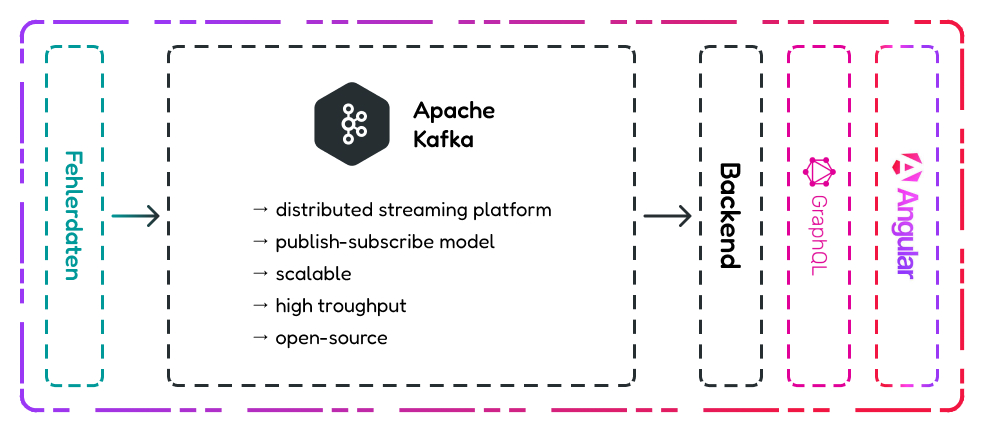
\includegraphics[width=1\textwidth]{content/img/Architecture/Architecture_Kafka.jpg}
    \caption{Architektur unseres Prototyps mit Fokus auf Kafka}
    \label{fig:KafkaArchitektur}
\end{figure}
\FloatBarrier

\subsection{Logik im Backend: Spring Framework}

Das Backend-System, das mit dem \emph{Java Spring Framework} entwickelt worden ist, ist für die Verarbeitung der empfangenen Daten zuständig, dies ist auch in der Darstellung \ref{fig:BackendArchitektur} zu sehen.  Mithilfe von \emph{Spring for Apache Kafka}, welches die Integration von Kafka in Spring ermöglicht, werden die Daten von Apache Kafka abgefragt und an das Backend weitergeleitet. In Spring werden diese Daten dann entsprechend verarbeitet und für die Speicherung in der Datenbank vorbereitet.

\begin{figure}
    \centering
    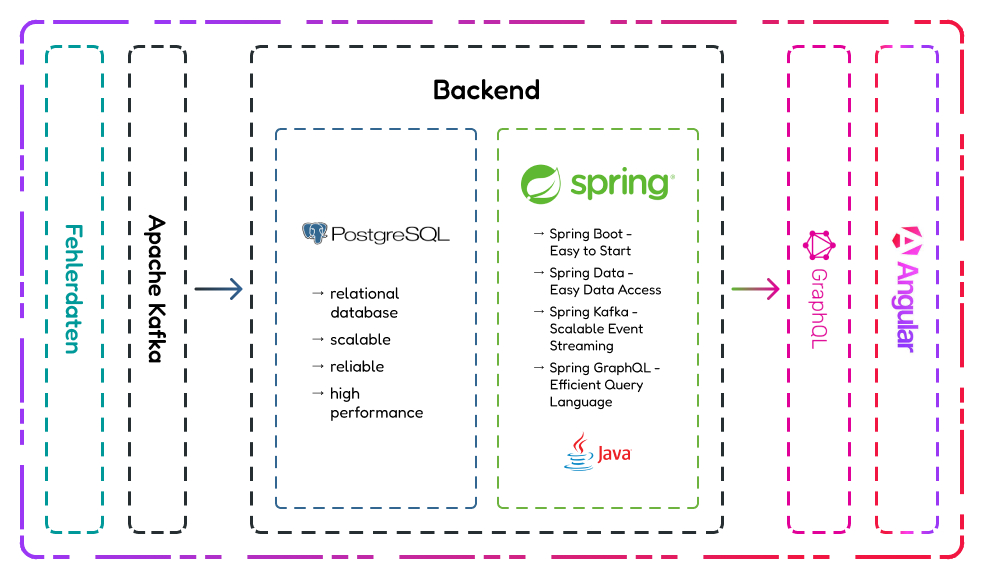
\includegraphics[width=1\textwidth]{content/img/Architecture/Architecture_Backend.jpg}
    \caption{Architektur unseres Prototyps mit Fokus auf das Backend}
    \label{fig:BackendArchitektur}
\end{figure}
\FloatBarrier

Die Entscheidung für Java als Programmiersprache und Spring als Application-Framework ist im Wesentlichen aus zwei Gründen gefällt worden. Einerseits ist die Verwendung von diesen Technologien eine fixe Anforderung seitens Siemens gewesen. Auf der anderen Seite bieten sie immense Vorteile für die Entwicklung der Anwendungen in Bezug auf unsere spezifischen Nutzungsszenarien. In den folgenden Abätzen werden diese Technologien vorgestellt und ihre Vorteile genauer beleuchtet.

Java ist eine objektorientierte, plattformunabhängige Programmiersprache, die ursprünglich von Sun Microsystems entwickelt worden ist und jetzt von Oracle Corporation gepflegt wird. Sie ist in den 1990er Jahren eingeführt worden und hat sich seitdem zu einer der beliebtesten Programmiersprachen entwickelt, insbesondere für die Entwicklung von Unternehmensanwendungen, Webanwendungen, mobilen Anwendungen und großen Systemen. \cite{javaDocs}

Ein wichtiges Konzept von Java ist die objektorientierte Programmierung (OOP). Das bedeutet, dass alles in Java als Objekt betrachtet wird. Objekte sind Instanzen von Klassen, die Daten und Methoden zur Manipulation dieser Daten enthalten. OOP-Konzepte wie Vererbung, Polymorphismus und Kapselung werden in Java stark unterstützt. Dadurch kann eine intuitive und effiziente Programmierung erreicht werden, was eine schnelle Entwicklung von Anwendungen ermöglicht. \cite{javaDocs}

Ein großer Selling-Point dieser Programmiersprache ist die Plattformunabhängigkeit. Java-Programme werden in Bytecode kompiliert, der auf der \emph{Java Virtual Machine (JVM)} ausgeführt wird. Dadurch sind Java-Anwendungen plattformunabhängig, was bedeutet, dass sie auf verschiedenen Betriebssystemen wie Windows, macOS und Linux ausgeführt werden können, solange eine JVM verfügbar ist. \cite{javaDocs}

Ein weiterer Vorteil ist die Unterstützung von \emph{Multi-Threading}, welches Anwendungen erlaubt, parallel mehrere Aufgaben abzuarbeiten. Dies ist besonders in Anwendungsfällen, welche eine große Last auf Anwendungssysteme ausüben, zum Beispiel bei Server-Systemen, von Vorteil. Außerdem hat Java ein reichhaltiges Ökosystem an Erweiterungen, wie zum Beispiel Frameworks oder Bibliotheken. Dies liegt daran, dass Java eine sehr große Popularität im Enterprise-Sektor geniest. Denn die Unternehmen, welche Java verwenden, unterstützen die Entwicklung von diesen Erweiterungen, damit ihre Produkte verlässlich und effektiv funktionieren. Aus all diesen Gründen ist die Verwendung von Java in Fall dieser Arbeit optimal. \cite{javaDocs,FireshipJava}

Das Java Spring Framework ist eine Erweiterung von Java, welche eine einfache Entwicklung von robusten, skalierbaren und wartbaren Anwendungen ermöglicht. Definitionsgemäß ist Spring ein \emph{Application-Framework} und ein \emph{Inversion of Control Container}. Ein Application-Framework ist ein strukturierter Satz von Bibliotheken, Komponenten und Tools, der die Entwicklung von Anwendungen erleichtert, indem er eine grundlegende Struktur und Funktionalität bereitstellt. Es werden komplexe Aspekte der Anwendungsentwicklung, welche grundsätzlich bei jeder Applikation gleich sind, wie der Netzwerk- oder Datenbankzugriff, abstrahiert. Damit kann der Fokus der Entwickler auf die eigentliche Anwendungslogik gelenkt werden und Ressourcen für die Erstellung von redundanten Komponenten eingespart werden. Um Probleme bei der Wiederverwendung zu vermeiden, wird auf das Konzept der Standardisierung gesetzt, welche eine zuverlässige Nutzung durch klar definierte Regeln schafft. \cite{springDocs}

Mit Inversion of Control ist eine Entwicklungstechnik gemeint, welche es ermöglicht, Objekte zu erstellen und ihre Abhängigkeiten dynamisch einzufügen. Dies fördert eine niedrige Kopplung zwischen den verschiedenen Komponenten einer Anwendung und erleichtert das Testen der Applikation. Das Java Spring Framework bietet in diesem Kontext die Umgebung an, welche das dynamische Auflösen und Einfügen von Abhängigkeiten in den Anwendungskomponenten ermöglicht. \cite{springDocs}

Der bedeutendste Vorteil in der Verwendung von Spring in Bezug auf diese Arbeit ist die leichte Integration von verschiedenen Technologien in die Anwendung durch die unzähligen Erweiterungen von diesem Framework. Beispielsweise ist die Einbindung der PostgreSQL Datenbank über die \emph{Spring Data JDBC} Bibliothek mit Leichtigkeit getätigt worden -- eine genauere Erklärung darüber ist im Kapitel \ref{postgresImpl}. Des Weiteren wird \emph{Kafka for Spring Framework} für das Interagieren des Backend-Systems mit Apache Kafka verwendet, welche auch eine Erweiterungsbibliothek ist -- eine detailreiche Erläuterung dazu ist im Kapitel \ref{apacheKafkaImpl}.

\subsection{Persistierung der Daten: PostgreSQL Datenbank}

Die verarbeiteten Daten werden in einer PostgreSQL-Datenbank persistiert. \emph{PostgreSQL} bietet eine robuste und leistungsstarke relationale Datenbanklösung, die die Anforderungen an die Datenspeicherung erfüllt. Das Java Spring Backend kommuniziert über Spring Data JDBC mit der Datenbank, um die Daten effizient zu speichern und abzurufen. Der ausschlaggebendste Grund zur Wahl von PostgreSQL ist die Anforderung von Siemens, dass eine relationale Datenbank verwendet werden soll, welche schon dem kooperierenden Entwicklungsteam von Siemens bekannt ist. Ein weiterer Grund ist die starke Popularität unter den Entwicklern und die starke Etablierung am Markt seitens PostgreSQL. In den nächsten Absätzen wird PostgreSQL und seine Vorteile genauer erklärt. 

PostgreSQL ist ein leistungsstarkes Open-Source-Datenbankmanagementsystem (DBMS), das auf dem objektrelationalen Datenbankmodell basiert. Außerdem unterstützt PostgreSQL Transaktionen, die es ermöglichen, eine Gruppe von Operationen als eine einzige atomare Einheit auszuführen. Das \emph{ACID}-Prinzip (Atomicity, Consistency, Isolation, Durability) wird unterstützt, was die Datenintegrität sicherstellt. Ein weiterer Vorteil von PostgreSQL ist, dass es in der Lage ist, als Hochverfügbarkeitsdatenbank zu operieren. Denn es können Daten zwischen mehreren Datenbankservern repliziert werden und somit kann bei einem Ausfall von einem DB-Server ein anderer die Arbeit übernehmen. 
Relationale Datenbanken haben ein sehr einfaches Konzept. Es ist aufgebaut auf Tabellen, welche Relationen zueinander haben, das heißt es können Zeilen aus verschiedenen Tabellen in Verbindung stehen, wobei jede Zeile eine Sache beschriebt. Beispielsweise könnte einer Person eine Adresse zugeordnet werden durch eine Relation zwischen einer Personentabelle und Adresstabelle. Jedoch haben relationale Datenbanken einen Haken, wenn die Daten zu stark vernetzt sind, dann kommt diese Technologie an seine Grenzen. Im Falle dieser Arbeit sind die zu verwaltende Daten Graphdaten, was stark vernetzte Daten sind, wie trotzdem eine effiziente Speicherung und performantes Abfragen gelungen ist, wird im Kapitel \ref{postgresImpl} beschrieben.  \cite{postgreSQLDocs, FireshipPostgreSQL}